
\documentclass{article}
\usepackage{amsmath}
\usepackage[margin=1in]{geometry}
\usepackage{amsfonts}
\usepackage{hyperref}
\usepackage{graphicx}
\usepackage{siunitx}
\usepackage{cancel}
\usepackage{xfrac}


\begin{document}
	
		\title{Green's Theorem}
	\author{Andy Chong Sam}
	\date{}
	\maketitle
	
	\section{Overview}
	
	\par\noindent Green's Theorem relates the curl of a vector field to the line integral along around a simply connected region. In the right circumstances it can greatly simplify the line integral calculation. In Figure 1, I and II meet the criteria but III and IV do not. Region III has a path inside of the main path whereas IV is not connected.
	\newline
	
	\begin{center}
		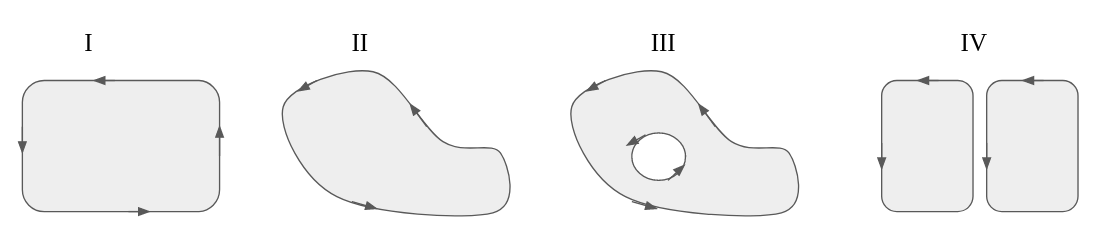
\includegraphics[width=10cm]{simply-connected.png}
	\end{center}

	\begin{center}
	Figure 1
\end{center}
	
	\par\noindent Given a field \(F=<P,Q>\) if R is a simply connected region with a boundary \(C\) oriented counterclockwise, and if \(P\) and \(Q\) have continuous first partial derivatives, then:
	
	\begin{flalign}
		\int_{C} P\;dx + Q\;dy = \int \int_{R}(\frac{\partial Q}{\partial x} - \frac{\partial P}{\partial y})\;dA
	\end{flalign}

	\section{Alternative Line Integral Notation}
	
	\par\noindent Before we Expression (1) let's explain the notation used on the left, \(P\;dx + Q\;dy\). We start with the formulation for line integrals along a path \(C\):
	
	\begin{flalign*}
		\int_{C}F\;dr = \int_{a}^{b} F(r(t)) \cdot r'(t)\;dt
	\end{flalign*}

	\par\noindent Let's suppose \(F=<P,Q>\), then developing the dot product would get us:
	
	\begin{flalign*}
		\int_{a}^{b} <P,Q> \cdot <x'(t), y'(t)>\;dt
	\end{flalign*}
	
	\begin{flalign*}
		\int_{a}^{b} Px'(t) + Qy'(t)\;dt = \int_{a}^{b}Px'(t)\;dt + \int_{a}^{b}Qy'(t)\;dt =
		\int_{a}^{b}P\;\frac{dx}{dt}\;dt + 		\int_{a}^{b}Q\;\frac{dy}{dt}\;dt 
	\end{flalign*}

	\begin{flalign*}
		\int_{C} P\;dx + Q\;dy
	\end{flalign*}

	\par\noindent The use of this notation does not affect the calculation, but it does help with organization. Line integral and Green's Theorem problems are often presented in this format.
	
\end{document}